\question IP分组头部中有两个有关长度的字段,一个是头部长度字段,另一个是总长度字段,其中
\par\fourch{头部长度字段和总长度字段都是以8bit为计数单位}{头部长度字段以8bit为计数单位,总长度字段以32bit为计数单位}{\textcolor{red}{头部长度字段以32bit为计数单位,总长度字段以8bit为计数单位}}{头部长度字段和总长度字段都是以32bit为计数单位}
\begin{solution}前面已经用一句话来记住各个字段的计数单位,这句话是:不要总拿1条假首饰来骗我吧=不要总拿1条假首4来偏我8,从这一句话中可以得出总长度的计数单位是1B(8bit),首部长度的计数单位是4B(32bit),位偏移的计数单位是8B。
\end{solution}
\question 在IP首部的字段中,与分片和重组无关的是( ) 注:假设现在已经分片完成
\par\twoch{\textcolor{red}{总长度}}{标识}{标志}{片偏移}
\begin{solution}在IP首部中,标识域的用途是让目标主机确定一个新到达的分段属于哪一个数据报,用于重新组合分片后的IP数据报;而标志域中的DF(是否不能分片)和MF(是否后面还有分片)位都与分片有关;片偏移则是标志分片在IP数据报中的位置,重新组合分组的时候用到。
\end{solution}
\question 假设有一个B类地址指定了子网掩码255.255.255.0,则每个子网可以有的主机数为
\par\twoch{256}{\textcolor{red}{254}}{1024}{1022}
\begin{solution}由于B类地址的默认子网掩码是255.255.0.0,而题目给的子网掩码为255.255.255.0,可以看出从主机位拿了8位出来划分子网,最后只剩下8位来表示主机位,一共有256(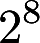
\includegraphics[width=0.14583in,height=0.15625in]{texmath/b618a75Cdpi7B3507D25E8})种可能,再去掉全``0''和全``1''的地址,所以每个子网可以有的主机数为254。
\end{solution}
\question 以太网的数据帧封装如图3-2所示,包含的TCP段中的数据部分最长应该是( ~)

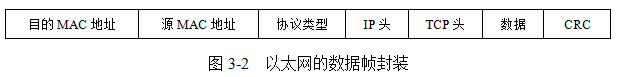
\includegraphics[width=3.33333in,height=0.40625in]{computerassets/25d66fd7ecf9a4aa73d66c4295ed68fb.png}
\par\twoch{1434}{\textcolor{red}{1460}}{1480}{1500}
\begin{solution}以太网帧数据域最大长度为1500B,而IP头和TCP头字段最小长度为20B。因此,用户数据最长为(1500-20-20)B=1460B。
\end{solution}
\question 在子网192.168.4.0/30中,能接受目的地址为192.168.4.3的IP分组的最大主机数是(
~)
\par\twoch{0}{1}{\textcolor{red}{2}}{4}
\begin{solution}在网络192.168.4.0/30中只有两位主机号,取值范围如下(为了简便,二进制和十进制混合用):

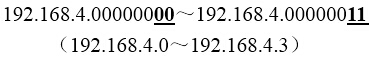
\includegraphics[width=3.84375in,height=0.59375in]{computerassets/a6b4274f028044f3f47aca2ecffced63.jpeg}

可以发现192.168.4.3恰好是其广播地址(广播地址的概念就是主机号全为``1'')。既然是广播地址,所以只要是在此网络内的主机,全部都可以接收到广播地址所发出的IP分组。而此网络一共有两个主机(4-2=2,要去掉全``0''和全``1'')。
\end{solution}
\question 某主机的IP地址为180.80.77.55,子网掩码为255.255.252.0。若该主机向其所在子网发送广播分组,则目的地址可以是(
)
\par\twoch{180.80.76.0}{180.80.76.255}{180.80.77.255}{\textcolor{red}{180.80.79.255}}
\begin{solution}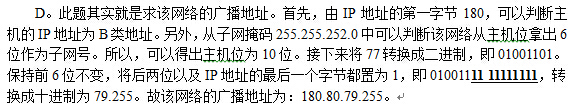
\includegraphics[width=5.98958in,height=1.12500in]{computerassets/9c47546d83511a0705eea3616ef8d8a5.jpeg}
\end{solution}
